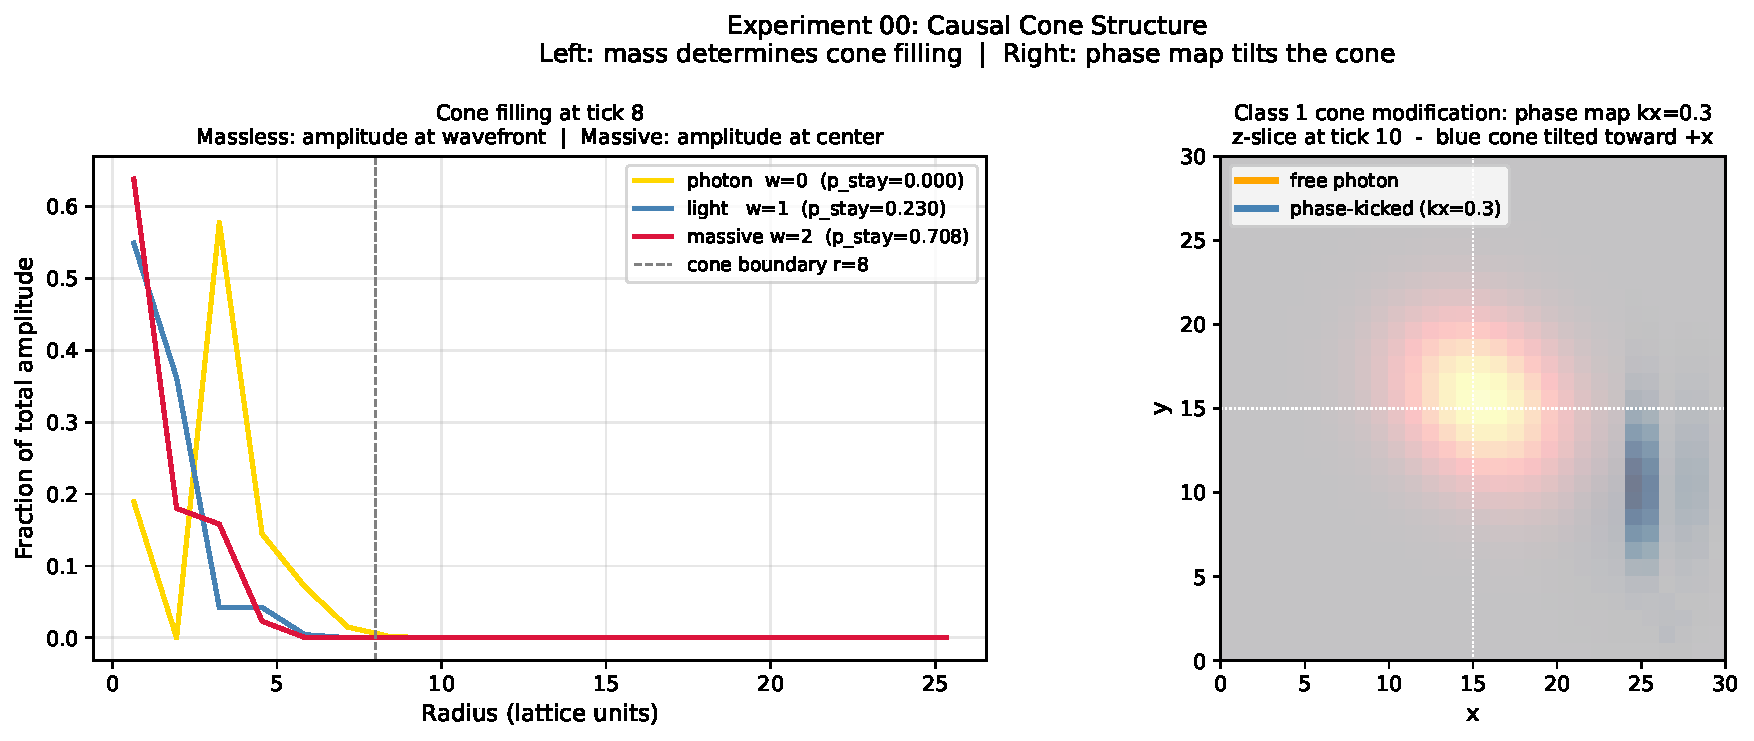
\includegraphics[width=\textwidth]{../figures/exp_00_cone_structure}
\caption{Causal cone structure on the $\Tdiamond$ lattice.
\textbf{Left:} Radial amplitude profile $P(r)$ at tick $t=8$ for three
particles distinguished by their instruction frequency $\omega$ (labeled
\texttt{w}).  The parameter $p_\text{stay} = \sin^2(\omega/2)$ is the
fraction of amplitude that remains interior to the wavefront each tick;
it serves as the lattice mass proxy.  A massless photon ($\omega=0$,
$p_\text{stay}=0$) concentrates its amplitude at the causal boundary
$r = t$, while massive particles ($\omega > 0$) retain a growing interior
fraction that converges toward $p_\text{stay}$ over time.
\textbf{Right:} $z$-slice of the probability density at tick $t=10$
for a free Gaussian wavepacket (orange, \emph{free photon}) and an
identical wavepacket to which a linear phase gradient
$\varphi(x) = k_x(x - x_0)$ with $k_x = 0.3$ was applied before
evolution (\emph{phase\_kicked}, blue).  The phase map shifts the
centre-of-mass by $\Delta x \approx 9.6$ lattice nodes toward $+x$,
demonstrating Class~1 cone modification: a spatially varying phase
imprinted on the wavefunction tilts the causal cone without violating
the $A=1$ constraint.}
